\documentclass[10pt]{article}
\usepackage[usenames]{color} %used for font color
\usepackage{amssymb} %maths
\usepackage{amsmath} %maths
\usepackage[utf8]{inputenc} %useful to type directly diacritic characters
\usepackage[letterpaper, portrait, margin=1.5in]{geometry}
\usepackage{booktabs}
\usepackage{graphicx,wrapfig}
\begin{document}
\subsection*{MSDS600 Week 2 Assignment - Nathan Worsham}
Examining the AFINN files, they are self described as “a list of English words rated for valence with an integer between negative five and positive five.” Also that the "words have 
been manually labeled” by a single author. According to Wikipedia, one meaning of valence, especially relating to psychology is to "characterize and categorize specific emotions”. I believe this to be the intention of this file—to assign values to the words so to capture (numerically) the mood or attitude of the text. Taking a sample of the words assigned a degree from -5 to 5, I consider the grouping of the words into values as a mostly subjective task. I do however agree that assigning higher or lower values to certain words is appropriate when they are taken in comparison. An example of this would be that “outstanding” has a more positive connotation to it versus “nice”. Although the data is numerical, it is a grouping of words at each numerical level. It would seem that the data type is ordinal, but by assigning values, the ordinal data attempts to take on quantitative attributes. There are order to the groupings, but there is no way to say how much more of a degree the word “hurrah" is over “amazing”. There are issues with this methodolgy however such as when language is taken out of context (in the case of quoting or re-tweeting), is sarcastic, is cynical, is slang, is an idiom, or other possible colloquialisms. \\ 

\begin{figure}[!h]
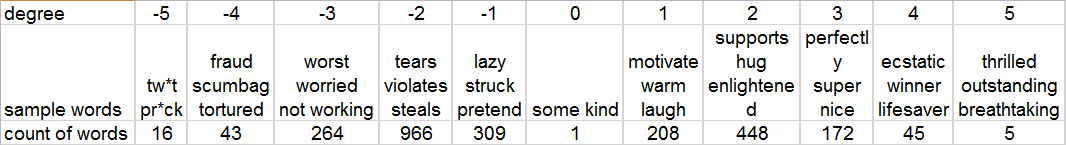
\includegraphics[scale=0.37]{table1.png}
\centering
\end{figure}

Looking at the data of the AFINN file, it shows that their are more negative words than positive (1598 vs 878 almost 2 to 1 margin), which would seem could potentially indicate or result in a bias towards a negative mood. However the twitter feed I captured ended up with results leaning in the positive direction: 
\begin{verbatim}
-5 sentiments  16 
-4 sentiments  121 
-3 sentiments  182 
-2 sentiments  254 
-1 sentiments  417 
 0 sentiments  0 
 1 sentiments  307 
 2 sentiments  581 
 3 sentiments  397 
 4 sentiments  93 
 5 sentiments  2 
\end{verbatim}

To compute the mean, I took each value multiplied by its number of occurrences:  
\begin{verbatim}
16*-5 + 121*-4 + 182*-3 + 254*-2 + 417*-1 + 307*1 + 581*2 + 397*3
+ 93*4 + 2*5
\end{verbatim}
becomes: 
\begin{verbatim}
-80 + -484 + -546 + -508 + -417 + 307 + 1162 + 1191 + 372 + 10 = 1007
\end{verbatim}
Then summed the number of occurrences: 
\begin{verbatim}
16 + 121 + 182 + 254 + 417 + 307 + 581 + 397 + 93 + 2 = 2370 
\end{verbatim}
And finally divided the sum by the count: 
\begin{verbatim}
1007/2370 = 0.4248945147679325 
\end{verbatim}

I was able to run this into R by using the following command: 
\begin{verbatim}
sentiment <- c(rep(-5,16),rep(-4,121),rep(-3,182),rep(-2,254),
rep(-1,417),rep(1,307),rep(2,581),rep(3,397),rep(4,93),rep(5,2)) 
\end{verbatim}

Which I could then run the summary function to confirm my results 
\begin{verbatim}
 summary(sentiment) 
  Min.   1st Qu.    Median      Mean   3rd Qu.      Max. 
-5.000000 -1.000000  1.000000  0.424895  2.000000  5.000000  
\end{verbatim}

So the Mean is slightly in the positive direction. According to the AFINN scale, the Mean would seem to indicate that during the timeframe I recorded the twitter feed that the trend of sentiment/mood/attitude of tweets made were slightly more of a positive sentiment than of a negative sentiment. This does seem to agree with the values I received as there was a total of 1380 positive comments versus 990 negative comments. Calculating the Mean makes the assumption that the values of the grouping of words is quantitative and more specifically interval data. It cannot be ratio data because it does not have a zero point (usablestats, n.d.). There is one value at zero--"some kind"--but this seems more like an error in the scale than a true zero value. If there were true zero values in the scale I would think the majority of words would fall here because it is the midpoint of the -5 to 5 range, instead the majority of the words in the AFINN scale fall on -2. 
Calculating the data as interval is problematic though because as mentioned earlier the grouping of the words is subjective as words don't have measurable differences and scoring unrelated words at the same value (such as "tears" and "steals") is difficult to defend. However calculating the Mean is not without significance as it does seem to help describe the direction of the data set based on the AFINN scale. Although there were 1380 positive responses, the Mean helps take into account the 990 negative responses when trying to show a trend.\begin{wrapfigure}{r}{5cm}
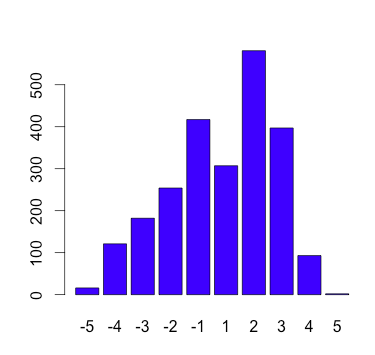
\includegraphics[width=5cm, scale=0.3]{barplot_week3.png}
\end{wrapfigure} On my twitter capture the Median was 1, and the Mode was 2. The Mean is below the Median making this a left-skewed distribution data set but because the distribution converges on the right (or positive side) the Mean is correctly showing this relationship. However the relationship is better seen by providing the Mean, Median, and Mode together or even visually:

If different words were used in the AFINN.txt file, undoubtedly the results would change and the analysis could change with it. To compensate for this, one could increase the sample size. As the stated from the Encyclopedia of Mathmatics (2012) about the Law of Large Numbers "the frequency of occurrence of a random event tends to become equal to its probability as the number of trials increases". So the larger the sample, the less of the chance of randomness will affect the outcome.

\subsection*{Reference}
Wikipedia, (n.d). Retrieved from https://en.wikipedia.org/wiki/Valence\_(psychology)\\*
Encyclopedia of Mathematics, (2012). Retrieved from\\* 
https://www.encyclopediaofmath.org/index.php/Law\_of\_large\_numbers
Usablestats (n.d.). Fundamentals of statistics 1: Basic concepts : Nominal, ordinal, interval and ratio. Retrieved from http://www.usablestats.com/lessons/noir

\end{document}